\documentclass[tikz,border=10pt]{standalone}
\usepackage{tikz}
\usetikzlibrary{arrows.meta,positioning,calc,3d}

\begin{document}
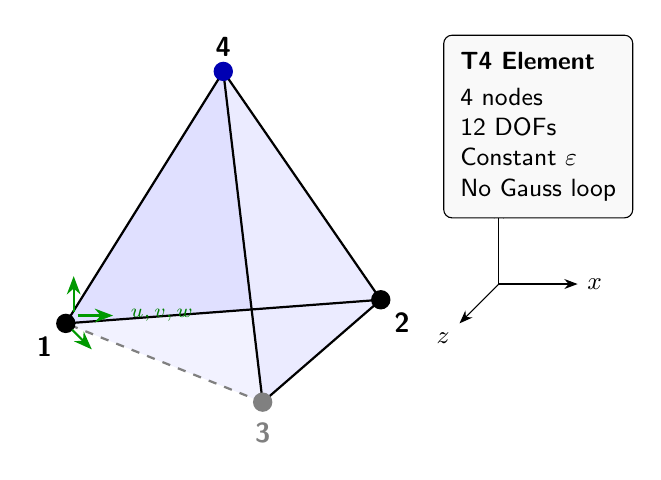
\begin{tikzpicture}[
    node font=\sffamily,
    >=Stealth,
    node dot/.style={circle, fill=black, inner sep=0pt, minimum size=7pt},
    node hollow/.style={circle, draw=black, fill=white, inner sep=0pt, minimum size=7pt, line width=1pt},
    dof arrow/.style={->, thick, color=green!60!black},
]

% Tetrahedron vertices
\coordinate (A) at (0,0);
\coordinate (B) at (4,0.3);
\coordinate (C) at (2.5,-1);
\coordinate (D) at (2,3.2);

% Back face (lighter)
\fill[blue!5] (A) -- (B) -- (C) -- cycle;

% Visible faces
\fill[blue!12] (A) -- (B) -- (D) -- cycle;
\fill[blue!8] (B) -- (C) -- (D) -- cycle;

% Edges
\draw[thick] (A) -- (B);
\draw[thick] (B) -- (C);
\draw[thick, dashed, gray] (C) -- (A);  % hidden edge
\draw[thick] (A) -- (D);
\draw[thick] (B) -- (D);
\draw[thick] (C) -- (D);

% Nodes
\node[node dot] (n1) at (A) {};
\node[node dot] (n2) at (B) {};
\node[node dot, fill=gray] (n3) at (C) {};  % back node
\node[node dot, fill=blue!70!black] (n4) at (D) {};

% Node labels
\node[below left=2pt, font=\bfseries] at (n1) {1};
\node[below right=2pt, font=\bfseries] at (n2) {2};
\node[below=4pt, font=\bfseries, gray] at (n3) {3};
\node[above=2pt, font=\bfseries] at (n4) {4};

% DOF arrows at node 1
\draw[dof arrow] (0.15,0.1) -- ++(0.45,0);
\draw[dof arrow] (0.1,0.15) -- ++(0,0.45);
\draw[dof arrow] (0.08,-0.08) -- ++(0.25,-0.25);
\node[font=\scriptsize, green!50!black, right] at (0.7,0.1) {$u,v,w$};

% Coordinate system
\begin{scope}[xshift=5.5cm, yshift=0.5cm]
    \draw[->] (0,0) -- (1,0) node[right, font=\small\itshape] {$x$};
    \draw[->] (0,0) -- (0,1) node[above, font=\small\itshape] {$y$};
    \draw[->] (0,0) -- (-0.5,-0.5) node[below left, font=\small\itshape] {$z$};
\end{scope}

% Info box
\node[draw, rounded corners=3pt, fill=gray!5, inner sep=6pt, font=\small, align=left] 
    at (6,2.5) {
    \textbf{T4 Element}\\[2pt]
    4 nodes\\
    12 DOFs\\
    Constant $\varepsilon$\\
    No Gauss loop
};

\end{tikzpicture}
\end{document}
